\section{Das IceCube-Experiment}
\label{sec:detector}
Der IceCube Detektor dient der Detektion von hochenergetischen 
Neutrinos und Myonen und besteht aus drei Komponenten: 
Dem IceTop Detektor, dem In-Ice Detektor welcher die gr\"o\ss te Komponente 
darstellt 
und dem DeepCore.
Das Experiment befindet sich am geographischen S\"udpol und die 
Hauptdetektionsschicht ist zwischen $\SI{1450}{\meter} - \SI{2450}{\meter}$ Tiefe
in einer klaren Eisschicht.
Mit Hilfe von Cherenkov Licht, welches mit 
5160 DOMs\footnote{digital optical modules} an 86 Strings detektiert werden kann, 
lassen sich hochenergetische geladene Teilchen detektieren.
Ein schematischer Aufbau ist in Abbildung \ref{fig:cube} gegeben.

\begin{figure}
  \centering
  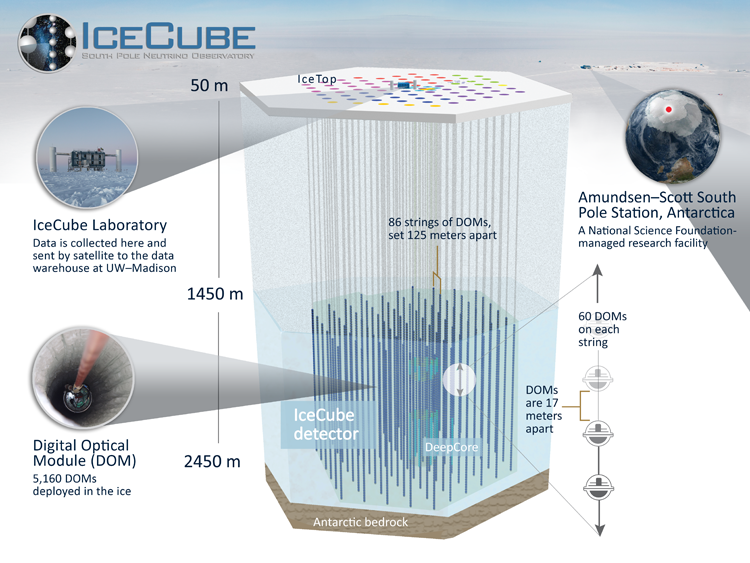
\includegraphics[width=0.8\textwidth]{plots/icecube_detector_sm.png}
  \caption{Schematischer Aufbau des IceCube Experiments \cite{IceCubeImage}.}
  \label{fig:cube}
\end{figure}

Der DeepCore besteht aus sieben Kabeln, 
welche sich im Zentrum des In-Ice Detektors befinden. 
Die Energieschwelle im In-Ice Detektor beträgt $\SI{10}{\giga\electronvolt}$.
Sie ist demnach deutlich geringer als die 
Energieschwelle von $\SI{100}{\giga\electronvolt}$ des In-Ice Detektors.
Das IceTop dient als Luftschauer 
Experiment welches Cherenkov Licht in lichtdichten Eistanks detektiert. 
Au\ss erdem kann es als Vetoregion f\"ur das In-Ice verwendet werden 
um gewisse Winkelbereiche auszuschlie\ss en.

Die Prozesse zur Detektion von Neutrinos geschehen 
\"uber Sekund\"arteilchen aus den schwachen Wechselwirkungen 
mit den Kernen im Eis als geladener Strom
\begin{equation*}
  \nu_l (\bar{\nu}_l) + A \to l^{\mp} + X
\end{equation*}
oder neutraler Strom
\begin{equation*}
  \nu_l + A \to \nu_l + X\,.
\end{equation*}

Hierbei verursachen Elektronen eine sph\"arischen Schauer aufgrund des rapiden 
Energieverlustes. Myonen hingegen haben einen eher langsamen Energieverlust 
und k\"onnen gr\"o\ss ere Distanzen \"uberwinden und haben eine lange "Lichtspur" 
als Signatur. Tau-Leptonen haben eine \"ahnliche Signatur wie Elektronen aufgrund 
ihrer geringen Lebensdauer.
Myonen erzeugen zu wenig Cherenkov Licht um detektiert zu werden aber sie 
generieren unter Anderem 
Photonen und $e^+ e^-$ Paare im Medium, welche selbst wieder schauern 
und weitere Elektron-Positron Paare erzeugen und von den 
PMT\footnote{Photomultipliern} detektiert werden, sofern die Geschwindigkeit 
der Sekundärteilchen schneller ist, als die Lichtgeschwindigkeit des 
Mediums.
